\subsection{Participatory Design}
\par  Working with researchers from three different scientific research groups, we identified the needs and challenges of scientific data analysis and potential opportunities for VQSs, via interviews and cognitive walkthroughs. We recruited participants by reaching out to research groups via email and word of mouth, who have experienced challenges in dealing with large amounts of data. We initially spoke to analysts from 12 different potential application areas and narrowed down to three use cases in astronomy, genetics, and material science for our participatory design study, based on their suitability for VQS as well as diversity in use cases. Six scientists from three research groups participated in the design of \zv. On average, participants had more than 8 years of research experience working in their respective fields. %\techreport{We list the participants in Table~\ref{participants}, and will refer to them by their anonymized ID as listed in the table throughout the paper.}
\par Given our early conversations with participants, we built a basic VQS to serve as the functional prototype in the design study. This early VQS prototype allowed users to sketch a pattern or drag-and-drop an existing visualization as a query, then the system would return visualizations that had the closest Euclidean distance from the queried pattern. The details of the system is described in \cite{Siddiqui2017,Siddiqui2017VLDB}, which focused on the system and scalability aspects of the VQSs.
	% \begin{figure}[ht!]
	% \centering
	% 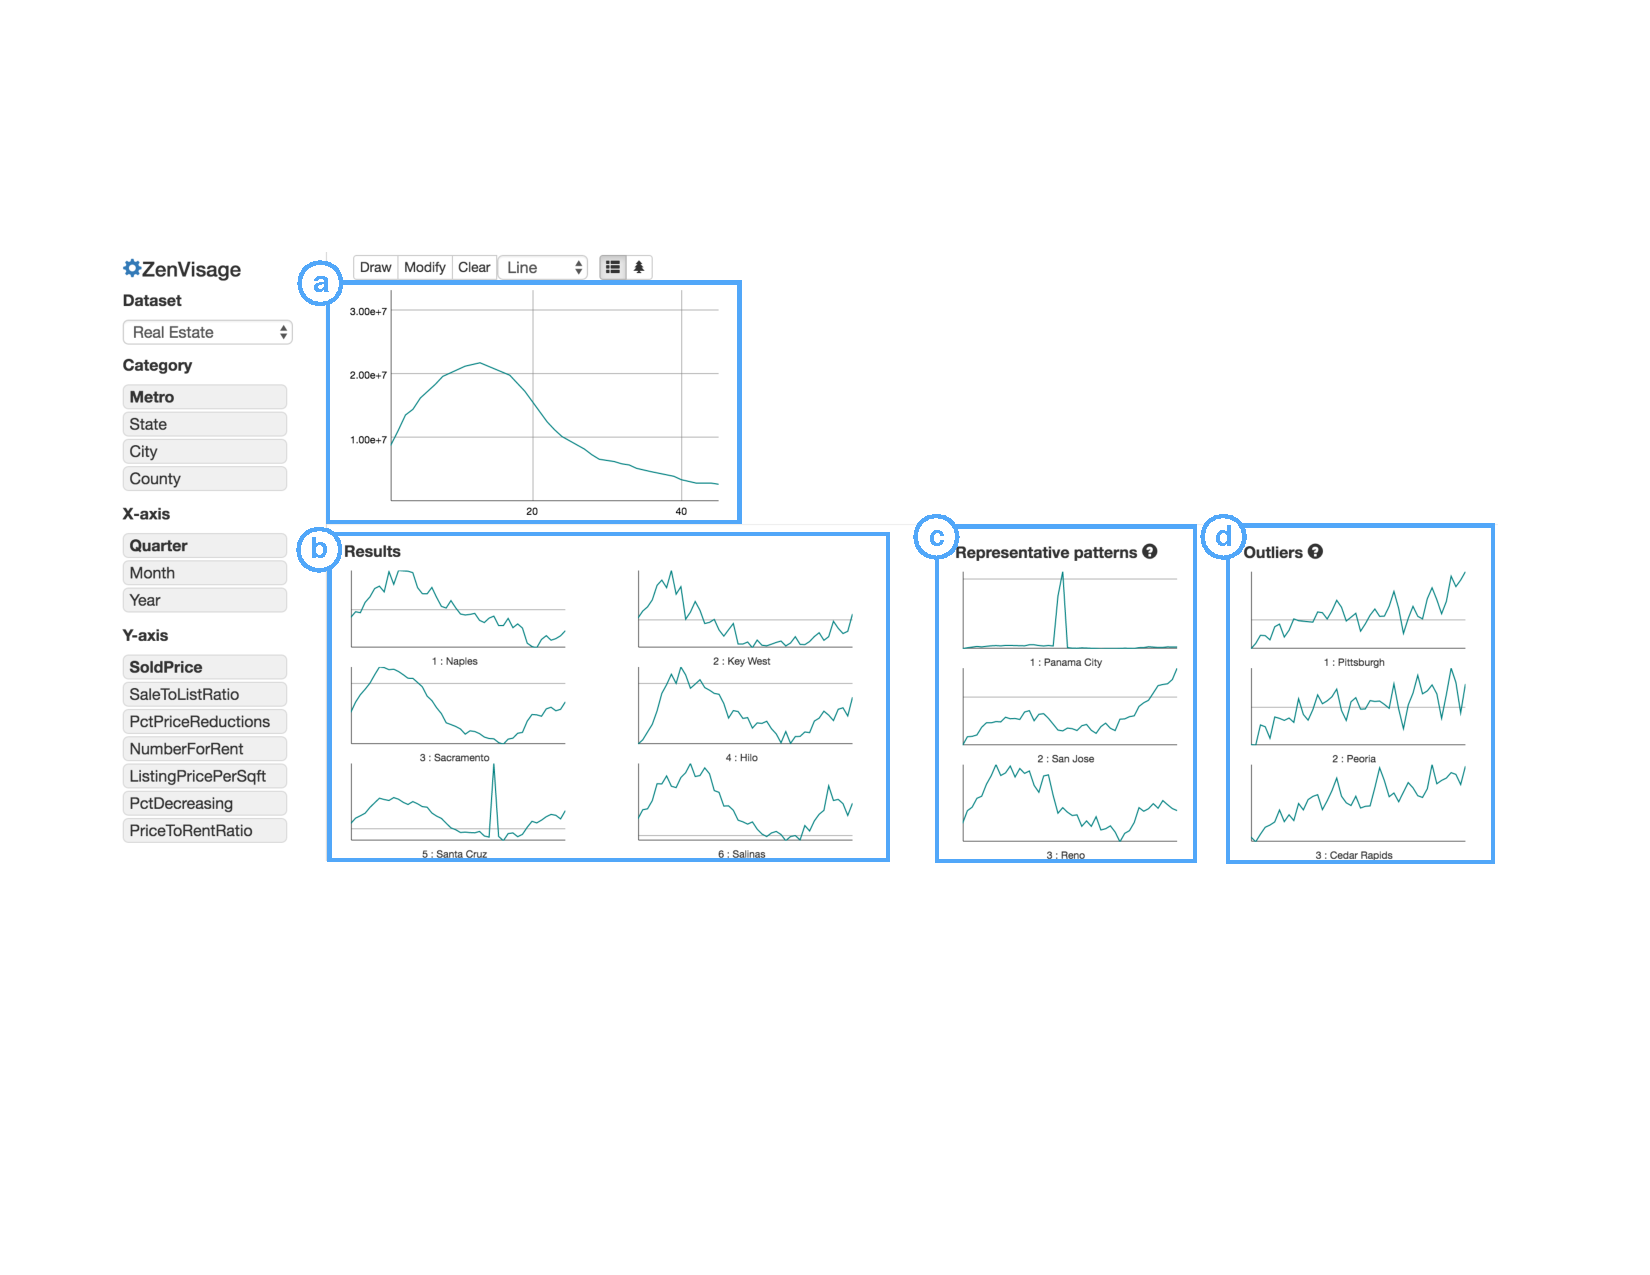
\includegraphics[width=\linewidth]{figures/oldZV_nozql.pdf}
	% \caption{The \zv prototype allowed users to sketch a pattern in (a), which would then return (b) results that had the closest Euclidean distance from the sketched pattern. The system also displays (c) representative patterns obtained through K-Means clustering and (d) outlier patterns to help the users gain an overview of the dataset.}
	% \label{oldZV}
	% \end{figure}
\par The use of functional prototypes is common and effective in participatory design to provide a starting point for the participants, as studied by Ciolfi et al.\cite{Ciolfi2016}. %For example, Ciolfi et al.\cite{Ciolfi2016} studied two different alternatives to co-design (starting with open brief versus functional prototype) in the development of museum guidance systems and found that while both approaches were equally fruitful, functional prototypes can make addressing a specific challenge more immediate and focused.
Our motivation for providing a functional prototype at the beginning of the participatory design sessions is to showcase capabilities of VQSs. Especially since VQSs are not common in the existing workflows of these scientists, participants may not be able to imagine their use cases without a starting point.
\par During the participatory design process, we collaborated with each of the teams closely with an average of two meetings per month, where we learned about their datasets, objectives, and how VQSs could help address their research questions. A summary timeline of our engagement with the participants and the features inspired by their use cases can be found in Figure \ref{timeline}. Participants provided datasets they were exploring from their domain, whereby they had a vested interest in using a VQS to address their own research questions. Through this process, we identified and incorporated more than 20 desired features into our VQS prototype, \zv, over the period of a year.
\begin{figure*}[!ht]
	\centering
	\captionsetup{justification=centering,margin=2cm}
	\vspace{-10pt}
	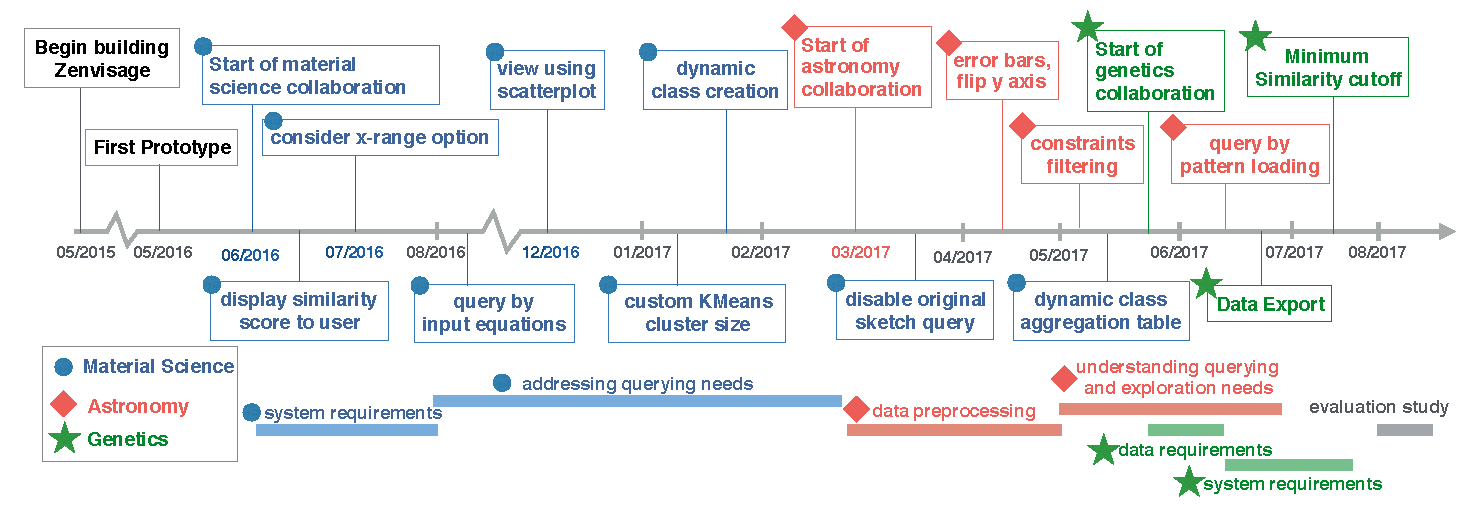
\includegraphics[width=6in]{figures/timeline_new.pdf}
	\vspace{-6pt}\caption{Participatory design timeline for the scientific use cases.}
	\label{timeline}
	\vspace{-10pt}
\end{figure*}